\chapter{Arquitetura do sistema}

A seguir os artefatos que serão gerados ao longo do desenvolvimento deste projeto e que servirão de suporte ao longo do processo de desenvolvimento.

\section{Modelagem funcional}
Nesta etapa são levantadas o Documento de Escopo, as e as Sprints Backlog.

\subsection{Documento de escopo}
Este é o ponto de início para desenvolvimento do projeto, nele deve ser descrito em alto nível, que tipo de problema este projeto resolve. A figura \ref{doc-escopo} mostra este documento.

\begin{figure}[H]
\caption{\label{doc-escopo} Documento de escopo}
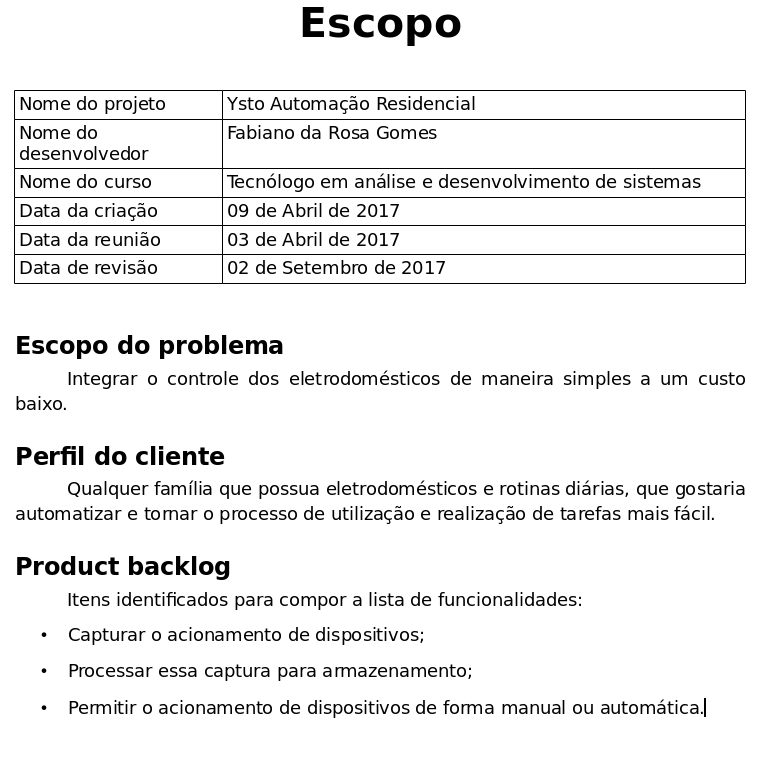
\includegraphics[scale=0.33]{img/escopo.png}
\legend{Fonte: Autor do projeto}
\end{figure}

\subsection{User Stories}
Este artefato faz a coleta, em um nível abstrato e sem riqueza de detalhes, das funcionalidades que os entes envolvidos no uso do sistema desejam que exista. Recebem um atributo identificador e uma descrição resumida, a tabela \ref{user-stories}.

\begin{table}[H]
   \caption{User Stories}
   \label{user-stories}
{
   \begin{tabularx}{\linewidth}{lX}
   \toprule
   Id & Descrição \\
   \midrule \midrule
   
    US001 & Como usuário do sistema eu gostaria de ligar ou desligar dispositivos, uma lâmpada por exemplo, usando meu Smartphone. \\

    US002 & Como usuário do sistema eu gostaria de saber quantos e quais dispositivos fazem parte da minha rede. \\

    US003 & Como usuário do sistema eu gostaria de saber a situação destes dispositivos, estão conectados? Em que estado estão? \\

    US004 & Como usuário do sistema eu gostaria de acessar meu perfil e verificar as ações que realizei em um período especifico de tempo. \\

    US005 & Como administrador do sistema eu gostaria de cadastrar outros usuários para a utilização do sistema. \\

    US006 & Como usuário do sistema eu gostaria de receber notificações no meu Smartphone sobre ações que estão ocorrendo em minha casa, mesmo estando fora dela. \\
   
   \bottomrule
   \end{tabularx}
}{
   \legend{Fonte: Produzido pelo autor}
}
\end{table}

A tabela \ref{product} mostra a listagem de User Stories, ordenada por prioridade.

\begin{table}[H]
   \caption{Product Backlog}
   \label{product}
{
   \begin{tabular}{ll}
   \toprule
   Id & Descrição \\
   \midrule \midrule
   
    US001 & Controlar o acionamento de dispositivos. \\
    US002 & Listagem de dispositivos. \\
    US003 & Status de dispositivos. \\
    US004 & Histórico de ações de usuários. \\
    US005 & CRUD de usuários. \\
    US006 & Notificações via Smartphone. \\

   \bottomrule
   \end{tabular}
}{
   \legend{Fonte: Produzido pelo autor}
}
\end{table}

\subsection{Sprints}
Aqui são listadas as sprints realizadas neste projeto, juntamente com suas revisões. Revisões estas que descrevem fatos ocorridos durante o desenvolvimento do projeto.

\paragraph{Sprint 1} A Sprint 1 iniciou com o desenvolvimento da US001, esta foi subdividida em tarefas mais detalhadas conforme a figura \ref{sprint-1}.

\begin{figure}[H]
\caption{\label{sprint-1} Detalhamento sprint 1}
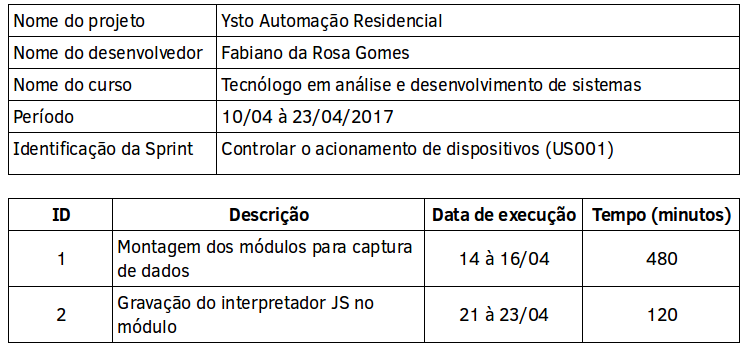
\includegraphics[scale=0.5]{img/sprint-1.png}
\legend{Fonte: Autor do projeto}
\end{figure}

\paragraph{Retrospectiva da Sprint 1} Realizado a montagem de placas auxiliares para fixação no protoboard , posteriormente esse circuito é utilizado para demonstrar o funcionamento dos módulos que coletam as informações e fazem os acionamentos. A figura \ref{ysto-preeview} mostra a etapa final de montagem.

\begin{figure}[H]
\caption{\label{ysto-preeview} Montagem das placas de fixação dos módulos}
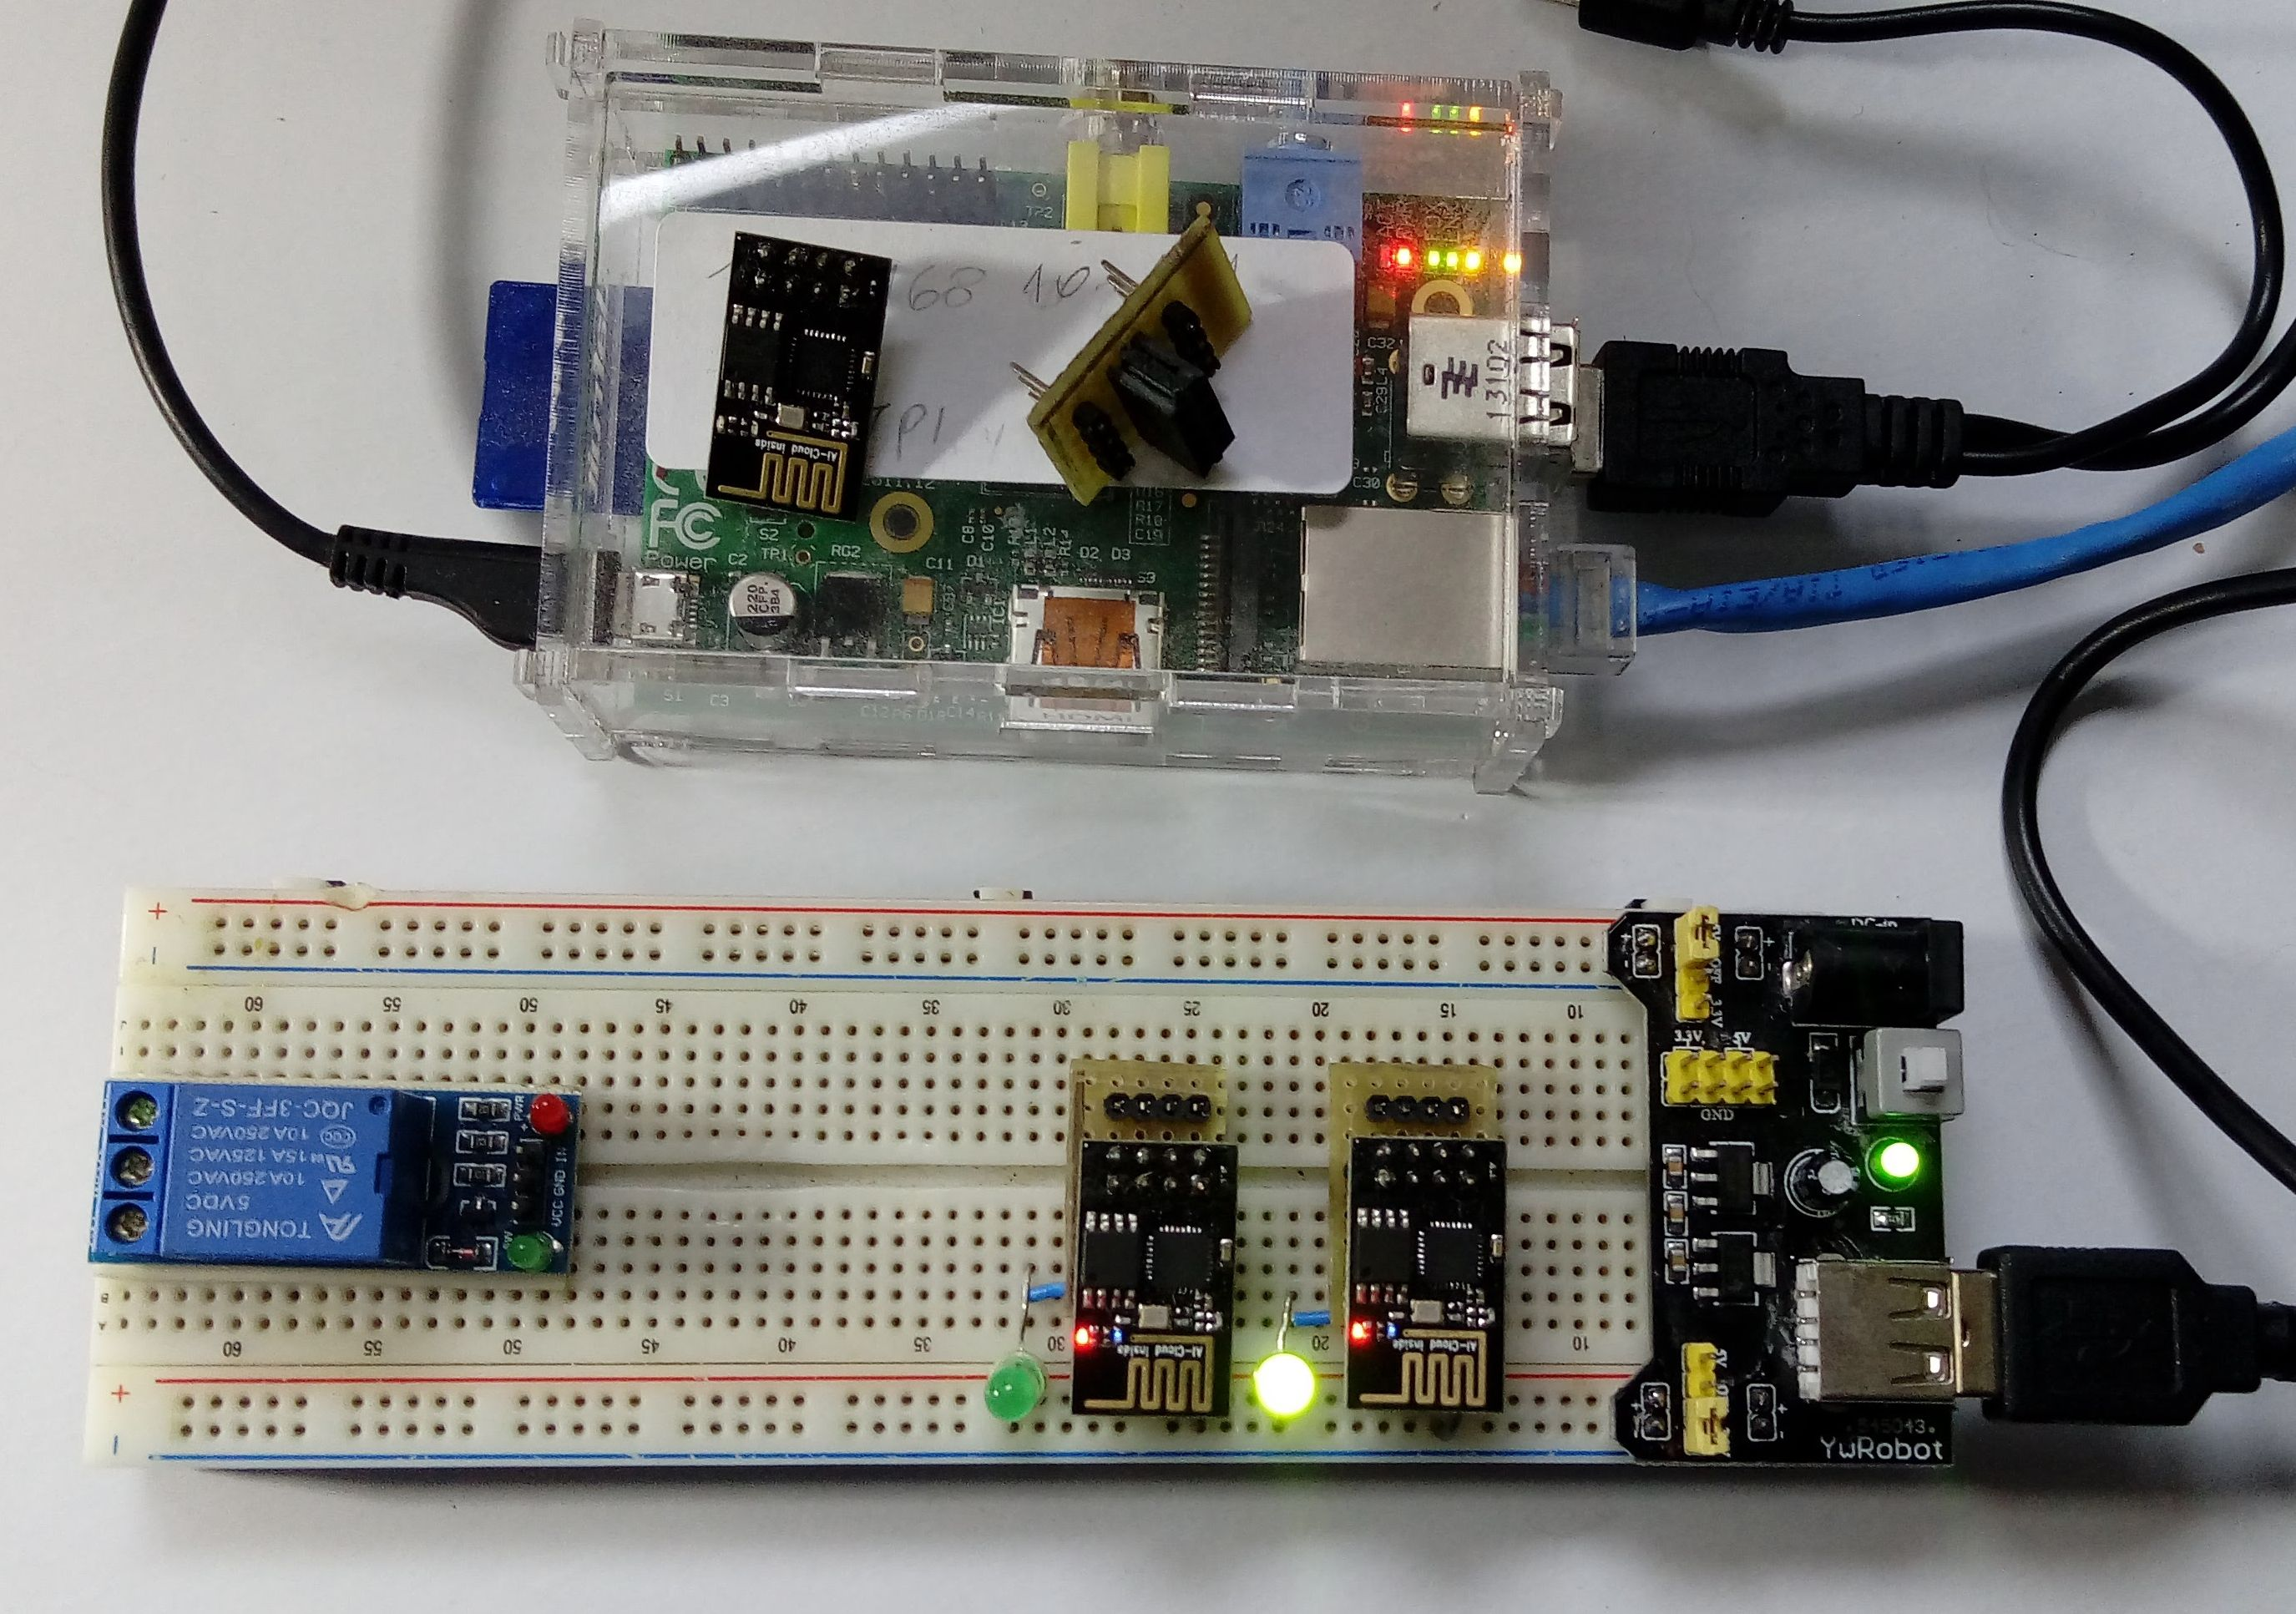
\includegraphics[scale=0.15]{img/ysto-preview.jpg}
\legend{Fonte: Autor do projeto}
\end{figure}

Na realização desta etapa, o modelo escolhido apresentou problemas no uso do interpretador de comando JavaScript, o Espruino(Espruino, 2017). Existe um Bug que não permite a gravação de informações na região não volátil de memória do módulo, isso inviabiliza temporariamente a utilização desta versão do módulo ESP8266. A figura \ref{ma-preeview} mostra como é o referido módulo.

\begin{figure}[H]
\caption{\label{ma-preeview} Módulo ESP8266 tipo 01}
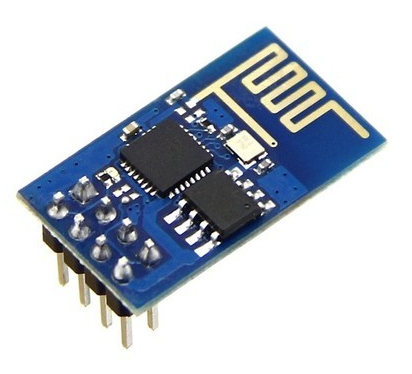
\includegraphics[scale=0.25]{img/esp8266-01.png}
\legend{Fonte: Website da Espressif}
\end{figure}

Este Bug foi relatado aos autores do projeto e após a correção é possível retomar o uso desta versão de hardware. Para dar continuidade ao projeto será utilizado uma variação de placa da família ESP8266, a tipo 12 ou também conhecida como Node MCU. A figura \ref{ma-novo-preeview} mostra como é esta placa.

\begin{figure}[H]
\caption{\label{ma-novo-preeview} Módulo ESP8266 tipo 12}
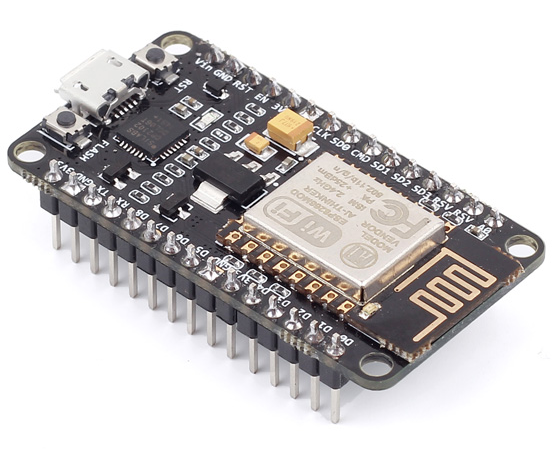
\includegraphics[scale=0.25]{img/esp8266-12.png}
\legend{Fonte: Website da Espressif}
\end{figure}

Este modelo não apresentou os problemas descritos anteriormente, nele temos mais capacidade de armazenamento e um número maior de General Purpose Input/Output.


\paragraph{Sprint 2} A Sprint 2 deu seguimento as atividades da US001, novas tarefas foram identificadas dentro deste contexto e adicionadas, conforme mostra a figura \ref{sprint-2}.

\begin{figure}[H]
\caption{\label{sprint-2} Detalhamento sprint 2}
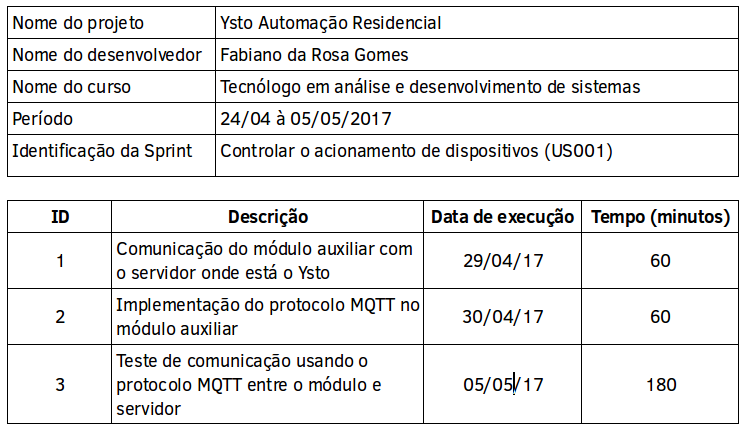
\includegraphics[scale=0.5]{img/sprint-2.png}
\legend{Fonte: Autor do projeto}
\end{figure}

\paragraph{Retrospectiva da Sprint 2} Realizado um teste com uma biblioteca disponibilizada para o framework Arduíno (Arduino, 2017), a ESPHelper (ESPHelper, 2017), com ela foi possível a utilização da placa ESP-01, mantendo as dimensões reduzidas do nosso módulo de acesso e captura de informações do mundo físico. Para a realização dos testes de comunicação com o servidor, já utilizando o lugar final onde este ficará armazenado, foi utilizado o cliente para o protocolo MQTT chamado Mosquitto (Mosquitto, 2017).

\paragraph{Sprint 3} Esta Sprint deve ser o encerramento do Firmware conforme a figura \ref{sprint-3} contempla as seguintes atividades.

\begin{figure}[H]
\caption{\label{sprint-3} Detalhamento sprint 3}
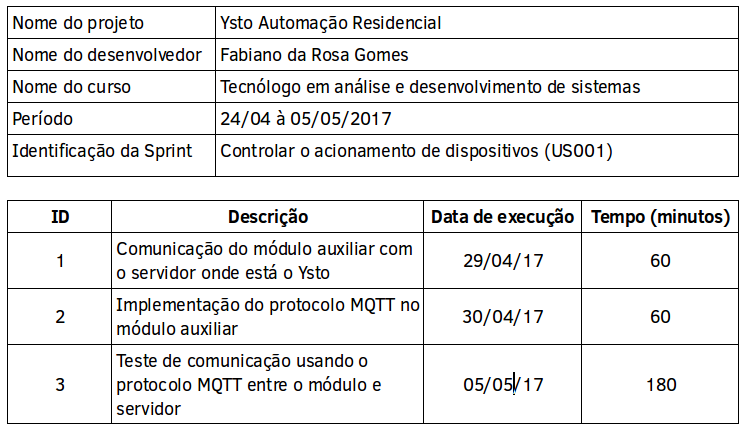
\includegraphics[scale=0.5]{img/sprint-2.png}
\legend{Fonte: Autor do projeto}
\end{figure}

\paragraph{Retrospectiva da Sprint 3} Realizado a implementação de acionamento do módulo auxiliar.

\paragraph{Sprint 4} A figura \ref{sprint-4} mostra o planejamento da sprint 4.

\begin{figure}[H]
\caption{\label{sprint-4} Detalhamento sprint 4}
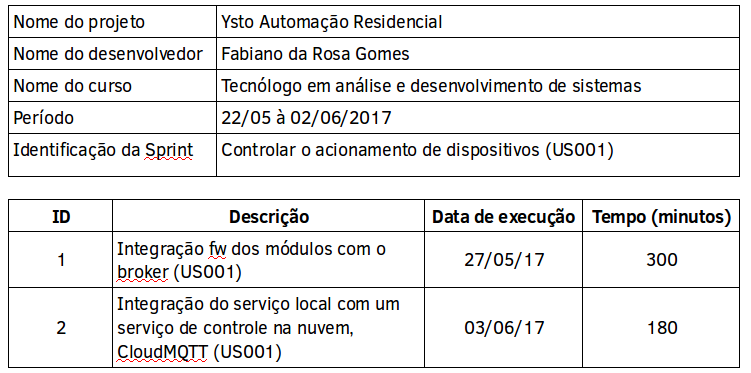
\includegraphics[scale=0.5]{img/sprint-4.png}
\legend{Fonte: Autor do projeto}
\end{figure}


\paragraph{Retrospectiva da Sprint 4} Nesta Sprint foi fixado uma estrutura de tópicos para controlar os Módulos Auxiliares (MA), também foi feita a ligação do serviço Mosquitto instalado na RaspberryPI com um serviço que roda na nuvem chamado CloudMQTT\footnote{https://www.cloudmqtt.com/}, isso permite controlar os módulo auxiliares em qualquer lugar onde existe acesso a internet.

\paragraph{Sprint 5} A figura \ref{sprint-5} mostra o planejamento da sprint 5.

\begin{figure}[H]
\caption{\label{sprint-5} Detalhamento sprint 5}
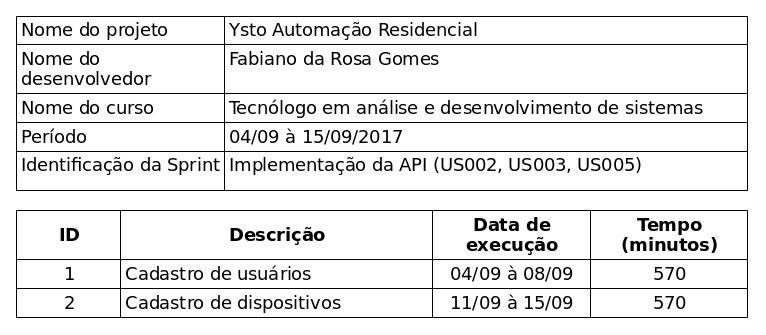
\includegraphics[scale=0.5]{img/sprint-5.png}
\legend{Fonte: Autor do projeto}
\end{figure}

\paragraph{Retrospectiva da Sprint 5} Nesta sprint ocorreu a implementação das US002, US003 e US005, em conjunto a esse desenvolvimento, testes unitários foram executados, a figura \ref{testes} mostra o relatório de testes realizados até o momento.

\begin{figure}[H]
\caption{\label{testes} Testes unitários da API}
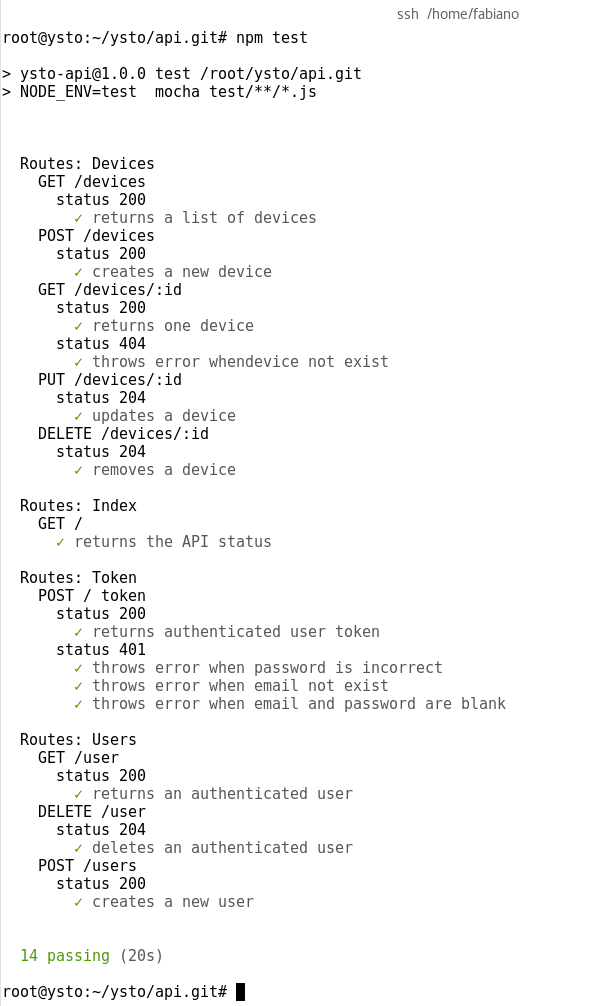
\includegraphics[scale=0.5]{img/resultado-testes.png}
\legend{Fonte: Autor do projeto}
\end{figure}

\paragraph{Sprint 6} A figura \ref{sprint-6} mostra o planejamento da sprint 6.

\begin{figure}[H]
\caption{\label{sprint-6} Detalhamento sprint 6}
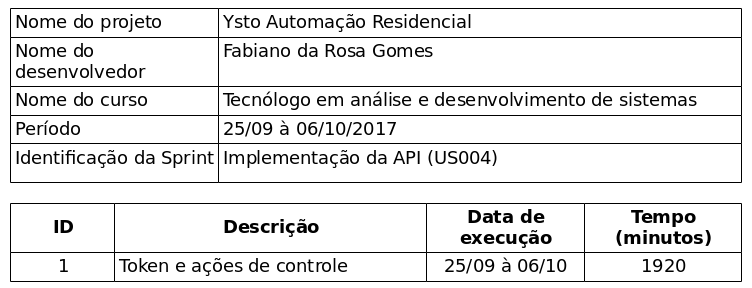
\includegraphics[scale=0.5]{img/sprint-6.png}
\legend{Fonte: Autor do projeto}
\end{figure}

\paragraph{Retrospectiva da Sprint 6}
Finalizamos a sprint 6 dentro do cronograma definido, todos os \textit{end-points} foram testados de forma automática.

\paragraph{Cancelamento da Sprint 7}
Na sprint 7 estava previsto a implementação da Interface com o usuário (UI), mas no decorrer de uso da API desenvolvida na sprint 6 problemas de performance foram percebidos, durante o período de pesquisa para entender o que estava acontecendo, o seguinte levantamento foi realizado:

\begin{itemize}
    \item[a]) Tempo de inicio de testes automáticos: 10 ~ 15 segundos;
    \item[b]) Tempo de resposta para um acionamento de módulo auxiliar: 5 ~ 8 segundos;
    \item[c]) Quantidade de arquivos necessários para o funcionamento da API (módulos do NodeJS); 10.537 entre módulos e aplicativo;
    \item[d]) Quantidade de espaço ocupado no cartão SD pela API, em bytes: 64MB de arquivos
\end{itemize}

Essa parece ser uma característica do NodeJS, que tem como lema "Baterias não inclusas". Essa politica tem seus prós e contras, depois de muito pesquisar pareceu ser a melhor alternativa trocar a tecnologia de desenvolvimento da API. Python foi escolhido, justamente por fazer uma proposta do tipo "Baterias inclusas", o que impacta na quantidade de bibliotecas externas que é necessária para fazer uma API RESt funcionar. Com a refatoração em Python a API reduziu para um tamanho de 200KB em arquivos, a figura \ref{tree-view-project} mostra como a arvore da aplicação ficou estruturada.

\begin{figure}[H]
\caption{\label{tree-view-project} Estrutura do projeto}
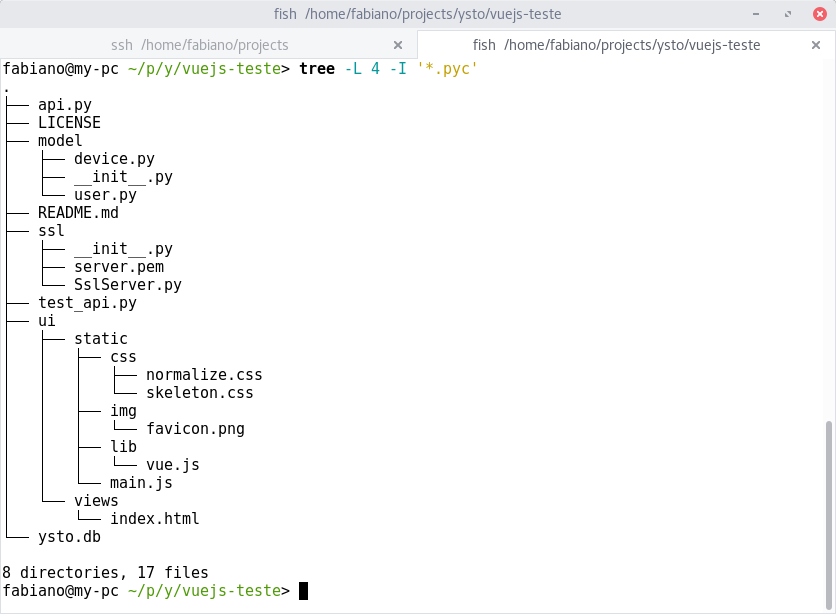
\includegraphics[scale=0.4]{img/tree-view.png}
\legend{Fonte: Autor do projeto}
\end{figure}

Além dos números e a simplicidade da estrutura do projeto, agora o acionamento de dispositivos é praticamente instantâneo (algo em torno de UM segundo entre a seleção da ação e o acionamento).

\paragraph{Cancelamento da Sprint 8}
Na sprint 8 estava previsto a finalização da UI, este trabalho foi iniciado, mas nos primeiros testes de integração com API foi percebido um problema de acesso aos recursos da API. A UI era um aplicativo que estava exposto na porta 3002 da central de controle e a API estava na porta 3001. Tanto o aplicativo cliente, no caso um browser quanto o servidor implementam politicas de segurança para evitar que ataques maliciosos possam comprometer o funcionamento de aplicativos pra internet, esta proteção basea-se no conceito conhecido como \textit{Cross-Origin Resource Sharing} (CORS).

Diversas tentativas foram feitas para fazer com que a API se tornasse disponível pra UI, dentre elas:

\begin{itemize}
    \item[a]) Do lado da UI envio de cabeçalhos com filtro aberto para domínios: Access-Control-Allow-Origin: *
    \item[b]) Do lado do servidor, permitir esta troca entre aplicativos do mesmo domínio;
    \item[c]) Instalação de servidores utilizados em aplicativos comerciais como o ngix e o lighttpd que possuem receitas para liberação do CORS;
    \item[d]) Instalação de extensões no browser para fazer a liberação de troca de mensagens entre aplicativos que ficam sob o mesmo domínio.
\end{itemize}

O fato é que nada disso funcionou, a opção final foi mesclar os dois aplicativos, desta forma a API e a UI agora são um projeto único e está disponível na porta 3001 da central de controle. A UI está na raiz do domínio <IP>/ e a API recebeu o seguinte endereço <IP>/api.

\paragraph{Sprint 7} A figura \ref{sprint-7} mostra o planejamento da sprint 7.

\begin{figure}[H]
\caption{\label{sprint-7} Detalhamento sprint 7}
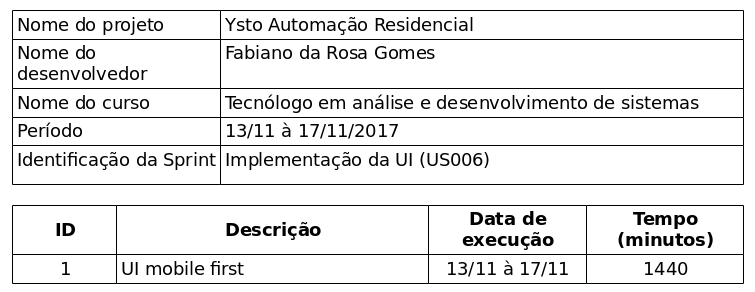
\includegraphics[scale=0.5]{img/sprint-7.png}
\legend{Fonte: Autor do projeto}
\end{figure}

\paragraph{Retrospectiva da Sprint 7}
Implementação realizada sem problemas, utilizado o template Skeleton \cite{SKELETON} para a criação da UI.

\paragraph{Sprint 8} A figura \ref{sprint-8} mostra o planejamento da sprint 8.

\begin{figure}[H]
\caption{\label{sprint-8} Detalhamento sprint 8}
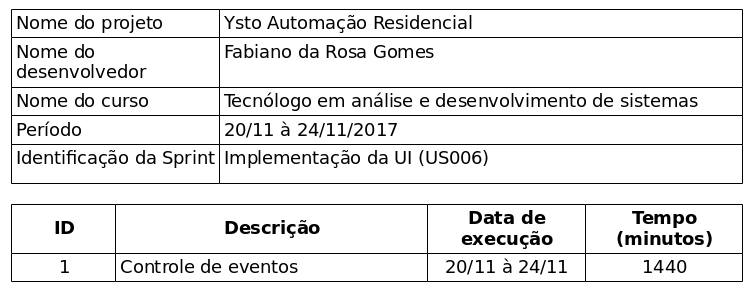
\includegraphics[scale=0.5]{img/sprint-8.png}
\legend{Fonte: Autor do projeto}
\end{figure}

\paragraph{Retrospectiva da Sprint 8}
TODO: Na data da impressão do relatório não havia executado esta sprint ainda.

\section{Modelagem do processo de negócio}
Diagramas de fluxo de dados, BPM, e Diagramas de sequência que descrevem o funcionamento do projeto.

\subsection{Firmware do módulo auxiliar}
O módulo auxiliar é o responsável pela interação do sistema com o mundo físico, cabe a ele fazer a leitura de input e o acionamento do output. O firmware responsável por fazer estas leituras e escritas está dividido em duas partes, a figura \ref{fw-acionamento} mostra como é feito o acionamento de uma carga.

\begin{figure}[H]
\caption{\label{fw-acionamento} Acionamento de carga}
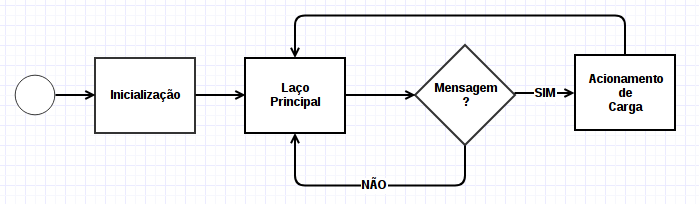
\includegraphics[scale=0.5]{img/fw-acionamento.png}
\legend{Fonte: Autor do projeto}
\end{figure}

Já a figura \ref{fw-leitura} mostra o que ocorre quando o módulo faz uma leitura.

\begin{figure}[H]
\caption{\label{fw-leitura} Leitura de dados}
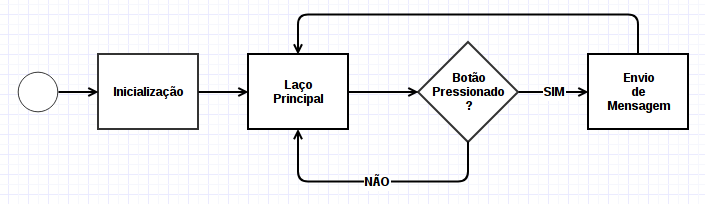
\includegraphics[scale=0.5]{img/fw-leitura.png}
\legend{Fonte: Autor do projeto}
\end{figure}

Para o desenvolvimento deste firmware foi definido que o pino 2 do ESP-01 será o responsável por acionar cargas e o pino 3 será o responsável pela leitura de dados.

\subsection{Controle de dispositivos através da API}
O controle dos dispositivos é feito através da API de controle, a figura \ref{api-acionamento} mostra uma sequência de acionamento de dispositivo.

\begin{figure}[H]
\caption{\label{api-acionamento} Acionamento através da API}
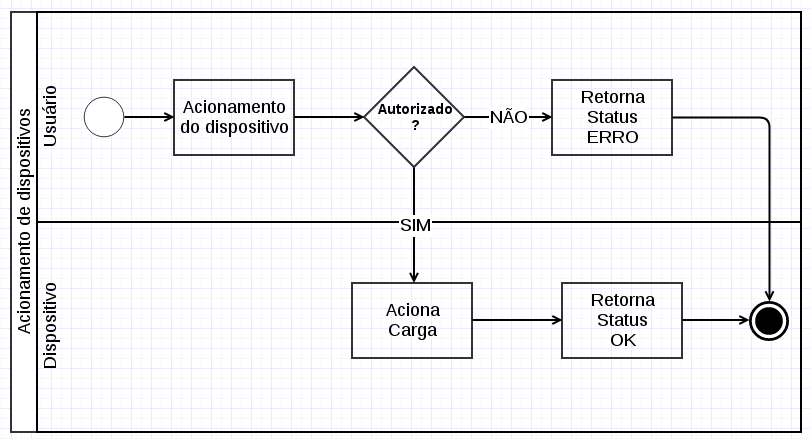
\includegraphics[scale=0.5]{img/acionamento-api.png}
\legend{Fonte: Autor do projeto}
\end{figure}

\section{Modelagem de dados}
Diagrama Entidade-Relacionamento e modelo conceitual.

\subsection{Modelagem da API}
Ysto usa uma Application Program Interface (API) que utiliza o padrão REST, segundo (Saudate, 2016, p.4):

\begin{citacao}
REST significa REpresentational State Transfer (ouTransferência de Estado Representativo, em tradução livre), e é um estilo de desenvolvimento de web services que teve origem na tese de doutorado de Roy Fielding (2000). Este, por sua vez, é coautor de um dos protocolos mais usados no mundo, o HTTP (HyperText Transfer Protocol). Assim, é notável que o protocolo REST é guiado (dentre outros preceitos) pelo que seriam as boas práticas de uso de HTTP:

a) Uso adequado dos métodos HTTP;

b) Uso adequado de URLs;

c) Uso de códigos de status padronizados representação de sucessos ou falhas;

d) Uso adequado de cabeçalhos HTTP e Interligações entre vários recursos diferentes.

O desenvolvimento desta API permite um maior desacoplamento de funções do sistema com a interface de uso.
\end{citacao}

\subsection{Definição de recursos}
Recursos são o ponto central de qualquer API REST, eles "são o conjunto de dados que trafegam pelo protocolo" (Saudate, 2016, p.5). Os chamados "verbos" do HTTP são utilizados como um padronizador de ações, sendo este procedimento uma excelente simplificação para ações repetitivas dentro de um sistema. As figuras que seguem, fazem justamente a ligação entre estes "verbos", POST, GET, PUT e DELETE com as ações que eles representam. A figura \ref{recurso-users} mostra como o recurso users é tratados dentro da API.

\begin{figure}[H]
\caption{\label{recurso-users} Recurso users na API}
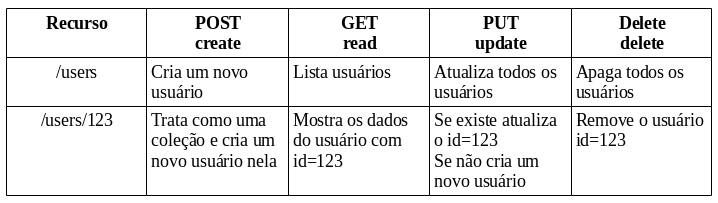
\includegraphics[scale=0.5]{img/recurso-users.png}
\legend{Fonte: Autor do projeto}
\end{figure}

A figura \ref{recurso-devices} mostra como o recurso devices é tratado dentro da API.

\begin{figure}[H]
\caption{\label{recurso-devices} Recurso devices na API}
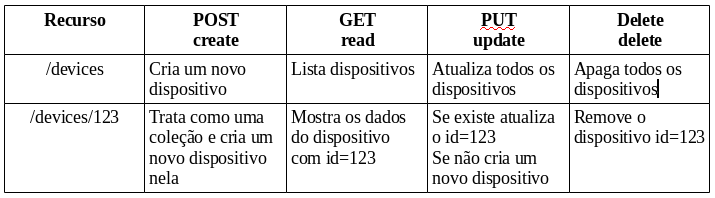
\includegraphics[scale=0.5]{img/resurso-devices.png}
\legend{Fonte: Autor do projeto}
\end{figure}

\subsection{Controle de acesso}
Todas as ações e recursos da API estão protegidas, o sistema de proteção para o uso deste sistema foi da adoção de tokens de segurança. Neste modelo de segurança, apenas mensagens devidamente assinadas chegam ao destino correto, executando a ação desejada. A figura \ref{controle-acesso} mostra como essa autenticação ocorre e como o usuário chega ao recurso desejado.

\begin{figure}[H]
\caption{\label{controle-acesso} Controle de acesso da API}
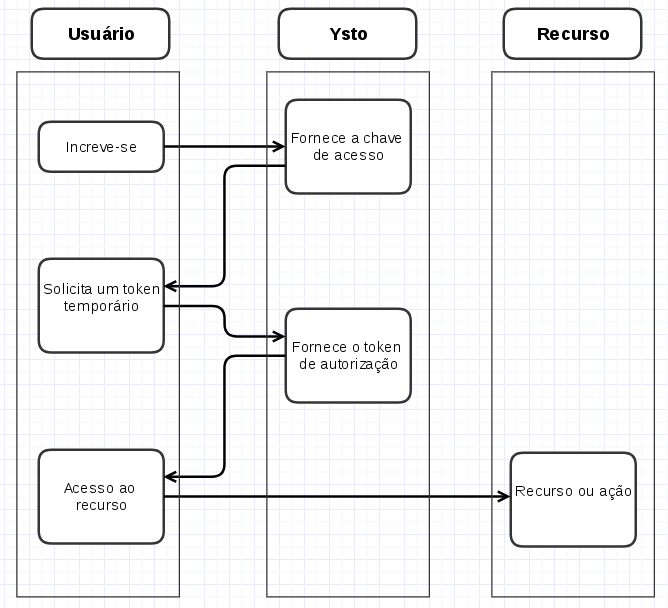
\includegraphics[scale=0.5]{img/auth-recursos.png}
\legend{Fonte: Autor do projeto}
\end{figure}

\subsection{Estrutura de mensagens}
No momento da solicitação de um recurso ou ação, temos um HTPP, a figura \ref{request} mostra a estrutura desta mensagem.

\begin{figure}[H]
\caption{\label{request} Solicitação ou request}
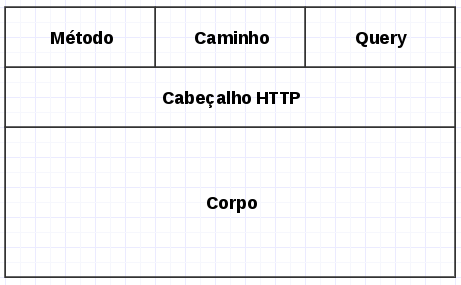
\includegraphics[scale=0.5]{img/api-request.png}
\legend{Fonte: Autor do projeto}
\end{figure}

Onde, cada campo poderia ser exemplificado da seguinte forma:

\begin{itemize}
    \item [a)] Método: GET, POST, PUT ou DELETE;
    \item [b)] Caminho: /api/v1/home/devices
    \item [c)] Query: ?search\&devices\&id=123
    \item [d)] Cabeçalho: Contém o token de acesso;
    \item [e)] Corpo quando necessário, em formato JSON JavaScript Object Notation.
\end{itemize}

A resposta a uma solicitação, obedece o padrão mostrado na figura \ref{response}.

\begin{figure}[H]
\caption{\label{response} Resposta ou response}
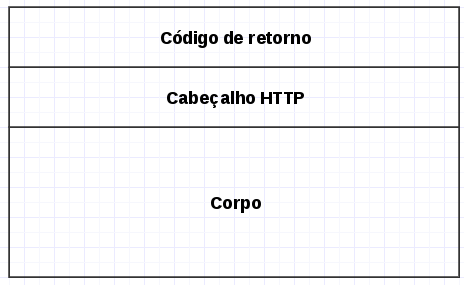
\includegraphics[scale=0.5]{img/api-response.png}
\legend{Fonte: Autor do projeto}
\end{figure}

\subsection{Código de status}
Dentro do modelo REST, os códigos de retorno do servidor são muito importantes e determinam em que estado nossa solicitação se encontra, esta é a conveção do protocolo HTTP (Saudate, 2016, p.27):

\begin{itemize}
    \item [a)] 1xx - Informacionais;
    \item [b)] 2xx- Códigos de sucesso;
    \item [c)] 3xx- Códigos de redirecionamento;
    \item [d)] 4xx- Erros causados pelo cliente;
    \item [e)] 5xx - Erros originados no servidor.
\end{itemize}

Dentro deste padrão esta API adota os seguintes valores de status para as requisições de recursos:

\begin{itemize}
    \item [a)] 200 OK Para operações realizadas com sucesso;
    \item [b)] 204 No Content Para operações de PUT, POST ou DELETE, onde o servidor pode se recusar a enviar contéudo;
    \item [c)] 400 Bad Request Resposta de erro genérico para qualquer erro de processamento;
    \item [d)] 401 Unauthorized Para solicitações não autorizadas ou com token de acesso inválido;
    \item [e)] 404 Not Found Para recursos que não existem no nosso contexto.
\end{itemize}

\section{Modelagem do banco de dados}
Para a interação com o banco de dados foi utilizado o ORM Sequelize e sendo que a atualização deste modelo se dá sempre que uma alteração nos modelos da aplicação ocorrem. A figura \ref{doc-devices} mostra como fica a estrutura do modelo que representa os devices.

\begin{figure}[H]
\caption{\label{doc-devices} Representção de devices}
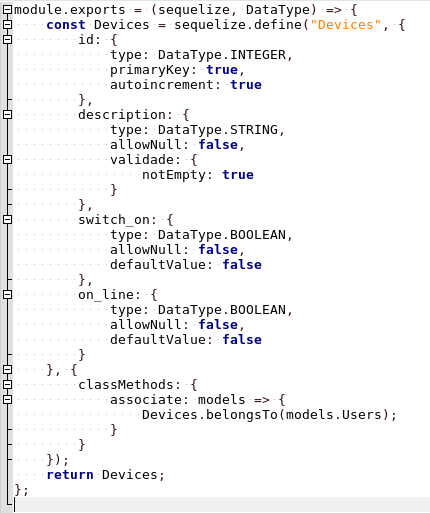
\includegraphics[scale=0.5]{img/devices-doc.png}
\legend{Fonte: Autor do projeto}
\end{figure}

Na figura \ref{doc-users} é exibido a estrutura que representa os Users.

\begin{figure}[H]
\caption{\label{doc-users} Representção de users}
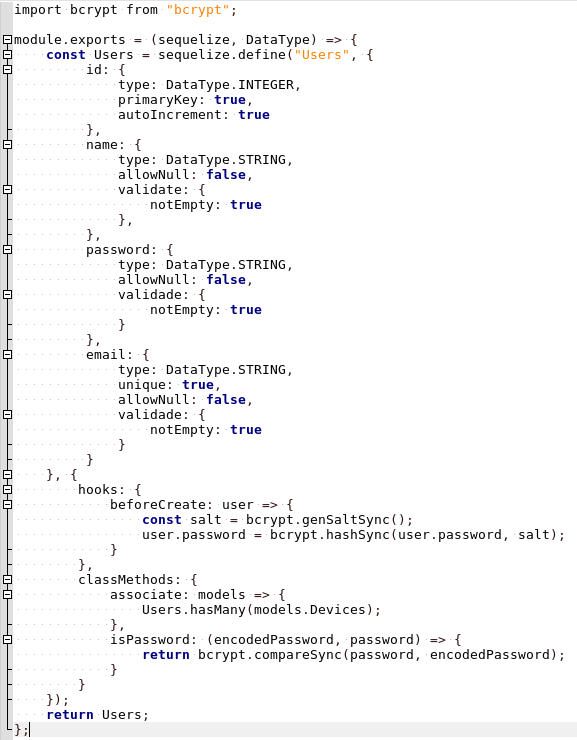
\includegraphics[scale=0.5]{img/users-doc.png}
\legend{Fonte: Autor do projeto}
\end{figure}

A modelagem ER (Entidade Relacionamento) do banco de dados é apresentada na figura \ref{er-db}.

\begin{figure}[H]
\caption{\label{er-db} ER do banco de dados}
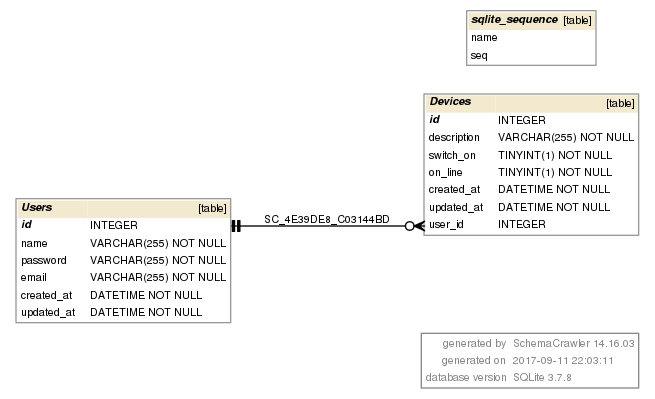
\includegraphics[scale=0.5]{img/ysto-db.png}
\legend{Fonte: Autor do projeto}
\end{figure}




